\paragraph{Kong}
\label{soa:tecnologias:kong}

Es una herramienta desarrollada por la empresa Mashape que permite la fácil administración de \glspl{acro:api}, centralizando el acceso a las mismas desde uno o más servidores que se encargan de llevar registro de qué servicios ofrecen, recibir los requerimientos para éstos y delegar la generación de las respuestas a los \glspl{term:backend} destinados a tal fin.

Kong funciona con una versión modificada de \nameref{soa:tecnologias:nginx}, haciendo las de \eng{proxy} reverso y proveyendo una estructura extensible mediante el uso de agregados (\eng{plugins}) para brindar funcionalidad adicional a la básica, como ser autenticación, registro en logs, limitación de datos (\eng{rate limiting}), \eng{caching}, por nombrar algunos. Toda su información se almacena en una base de datos no relacional Apache Cassandra, altamente escalable por naturaleza.

Básicamente, Kong se ubica entre los clientes y las instancias vivas de las \glspl{acro:api}, recibiendo los requerimientos para luego de aplicar las reglas que se le hayan especificado, enviarlos al servicio que corresponda.

\subparagraph{Licencia}

Kong está publicado bajo licencia Apache 2.0\footnote{La misma puede ser consultada accediendo a \url{https://getkong.org/license/}}.

\subparagraph{Extensiones disponibles (\eng{plugins})}

Este producto permite extender su funcionalidad y comportamiento básico mediante la adición de \eng{plugins} que brindan variadas funciones. Adicionalmente, en caso que necesitemos agregar comportamiento que no se encuentra disponible, podemos implementarlo nosotros mismos y contribuir nuestro propia extensión a la comunidad.

A continuación presentamos un breve listado de las extensiones que Kong ofrece actualmente:

\begin{itemize}
  \item \textbf{Autenticación:} Kong provee \eng{plugins} para agregar autenticación a las \glspl{acro:api} mediante distintas estrategias:
  \begin{itemize}
    \item \textbf{Basic:} Autenticación mediante usuario y contraseña. \\
    \url{https://getkong.org/plugins/basic-authentication}
    \item \textbf{Key:} Autenticación mediante una clave de \gls{acro:api}. \\
    \url{https://getkong.org/plugins/key-authentication}
    \item \textbf{OAuth 2.0:} Autenticación mediante el protocolo OAuth 2.0. \\
    \url{https://getkong.org/plugins/oauth2-authentication}
    \item \textbf{\gls{acro:hmac}:} Permite autenticar la identidad del cliente (\eng{consumer}) mediante firmas \gls{acro:hmac} en los mensajes. \\
    \url{https://getkong.org/plugins/hmac-authentication}
    \item \textbf{\gls{acro:jwt}:} Provee autenticación mediante el uso del estándar JSON Web Tokens. \\
    \url{https://getkong.org/plugins/jwt}
  \end{itemize}

  \item \textbf{Seguridad:} Las siguientes extensiones de Kong proveen capas adicinales de seguridad a los servicios:
  \begin{itemize}
    \item \textbf{\gls{acro:acl}:} Agrega listas de control de acceso para limiter qué consumers pueden acceder a qué \glspl{acro:api}. \\
    \url{https://getkong.org/plugins/acl}
    \item \textbf{\gls{acro:cors}:} Permite que se realicen requerimientos desde distintos dominios con las limitaciones que impongamos, algo ideal para la implementación de clientes puramente desarrollados en JavaScript que corran por completo en el navegador de los usuarios. \\
    \url{https://getkong.org/plugins/cors}
    \item \textbf{\gls{acro:ssl}:} Agrega la posibilidad de establecer conexiones verificables mediante la inclusión de certificados \gls{acro:ssl} a los servicios que proveemos, tanto individual como globalmente, sin necesidad de hacerlo en cada uno de los puntos de acceso de las \glspl{acro:api}. \\
    \url{https://getkong.org/plugins/ssl}
    \item \textbf{Restricciones por dirección IP:} Posibilita manejar listas blancas y listas negras de direcciones IP que pueden realizar requerimientos a nuestros servicios. \\
    \url{https://getkong.org/plugins/ip-restriction}
  \end{itemize}

  \item \textbf{Control de tráfico:} Estas extensiones habilitan reglas de control sobre el tráfico entrante y saliente de nuestras \glspl{acro:api}:
  \begin{itemize}
    \item \textbf{Límite de tasa de consulta (\eng{Rate limiting}):} Permite limitar la cantidad de requerimientos que un cliente puede hacer a los servicios en un periodo de tiempo dado. \\
    \url{https://getkong.org/plugins/rate-limiting}
    \item \textbf{Límite de tasa de respuesta (\eng{Response rate limiting}):} Hace posible limitar la cantidad de respuestas que los servicios envían en un periodo de tiempo dado (aplica límites sobre el tráfico saliente). \\
    \url{https://getkong.org/plugins/response-rate-limiting}
    \item \textbf{Límite de tamaño de solicitud (\eng{Request size limiting}):} Bloquea aquellos requerimientos cuyo cuerpo exceda un límite que especifiquemos en su tamaño. \\
    \url{https://getkong.org/plugins/request-size-limiting}
  \end{itemize}

  \item \textbf{Analíticas y monitoreo:} Tal vez el punto con menos opciones que provee Kong, ya que posee un único \eng{plugin} que agregue funcionalidad en este aspecto:
  \begin{itemize}
    \item \textbf{Galileo:} Integra el servicio de analíticas y monitoreo de \glspl{acro:api} Galileo, una plataforma paga de \eng{Business Inteligence} desarrollada por Mashape, los creadores de Kong. \\
    \url{https://getkong.org/plugins/galileo}
  \end{itemize}

  \item \textbf{Transformaciones:} Mediante estas extensiones, podemos realizar modificaciones a las peticiones o las respuestas de un servicio cuando pasa por Kong:
  \begin{itemize}
    \item \textbf{Transformación de peticiones (\eng{Request transformer}):} Modifica la solicitud antes de enviarla al servicio correspondiente. \\
    \url{https://getkong.org/plugins/request-transformer}
    \item \textbf{Transformación de respuestas (\eng{Response tranformer}):} Altera la respuesta obtenida desde la \gls{acro:api} antes de enviarla al cliente del servicio. \\
    \url{https://getkong.org/plugins/response-transformer}
  \end{itemize}

  \item \textbf{Registro de eventos (\eng{Logging}):} Estos \eng{plugins} permiten escribir a logs de registro las solicitudes y respuestas que pasan por Kong mediante distintas estrategias:
  \begin{itemize}
    \item \textbf{TCP:} Envía la información al log mediante una conexión realizada con un servidor que habla el protocolo TCP. \\
    \url{https://getkong.org/plugins/tcp-log}
    \item \textbf{UDP:} Ídem anterior, excepto que usando protocolo UDP. \\
    \url{https://getkong.org/plugins/udp-log}
    \item \textbf{HTTP:} \eng{Plugin} similar a los anteriores, excepto que lo hace contra un servidor que habla el protocolo HTTP. \\
    \url{https://getkong.org/plugins/http-log}
    \item \textbf{Archivo (\eng{File}):} Escribe la información en archivo local al servidor de Kong. \\
    \url{https://getkong.org/plugins/file-log}
  \end{itemize}
\end{itemize}

\subparagraph{Instalación y prueba}

Basándonos en los pasos detallados en la guía oficial de Kong\footnote{\url{https://github.com/Mashape/docker-kong}} para su instalación y ejecución mediante Docker\footnote{Desarrollar el potencial de Docker y las posibilidades que abre desde el punto de vista tanto de desarrollo de aplicaciones como de administración de las mismas en producción merecería un capítulo entero. Debido a que esto excede el alcance del presente trabajo, nos limitaremos a definir a Docker como una herramienta que permite ejecutar servicios (de cualquier tipo) en ambientes livianos aislados basados en GNU/Linux, los cuales ya empaquetan el servicio y cualquier dependencia que éste pudiera tener. Docker corre sobre un sistema operativo base que soporte la tecnología de contenedores (\eng{containers}). Para mayor información, se puede consultar el sitio oficial de Docker: \url{https://www.docker.com/what-docker}}, realizamos pruebas de concepto para analizar la factibilidad de implementación de esta herramienta, las cuales resultaron altamente satisfactorias. A continuación, reproduciremos las pruebas realizadas en el ambiente local\footnote{De ahí que todas las referencias a servicios que en estos pasos se realizan son utilizando \url{http://localhost}}, indicando los comandos ejecutados y las salidas obtenidas (en general acotadas a los datos relevantes para el caso). Para sintetizar los pasos, omitiremos la preparación del ambiente Docker, aunque se podría resumir simplemente en instalar dicha herramienta en el equipo donde se ejecutarán los contenedores.

Para iniciar los dos servicios requeridos por Kong para su funcionamiento (Apache Cassandra y Kong mismo), ejecutamos la siguiente secuencia de comandos:

\begin{listing}[H]
  \bashfile{src/02-capitulo-2/tecnologias/nodo-central/code/kong/00-preparacion.sh}
  \caption{Preparación y arranque de Kong}
  \label{soa:tecnologias:kong:bash-preparacion}
\end{listing}

Con el último comando comprobamos que el servicio está funcionando y que responde con la información de la instancia en ejecución, en formato \gls{lang:json}. Ahora que Kong está correctamente instalado y ejecutándose, podemos pasar a configurarlo y probar su funcionamiento.

Por defecto Kong atiende requerimientos en dos puertos diferentes:

\begin{itemize}
  \item \textbf{Puerto \texttt{8000}:} Aquí escucha la porción pública de Kong que funciona como proxy reverso de los servicios que registremos en él, proveyendo acceso a sus \glspl{acro:api}. A este puerto irán dirigidos todos los requerimientos de los clientes.
  \item \textbf{Puerto \texttt{8001}:} En este puerto Kong provee una \gls{acro:api} administrativa, mediante la cual se realizan todas las tareas de configuración y personalización de la herramienta. Esto implica varias cosas: por un lado, no necesitamos tener acceso por consola a los servidores donde corre el servicio de Kong, ya que simplemente con peticiones \gls{proto:http} basta para configurarlo; y por otro lado que necesitamos agregar políticas de seguridad adicionales para limitar el acceso a este puerto.
\end{itemize}

Teniendo esto en cuenta, procederemos a configurar una \gls{acro:api} de pruebas en Kong, utilizando el servicio online Mockbin\footnote{\url{http://mockbin.com}} que ofrece \glspl{term:endpoint} que imitan una \gls{acro:api} real para este tipo de situaciones.

\begin{listing}[H]
  \bashfile{src/02-capitulo-2/tecnologias/nodo-central/code/kong/01-agregar-mockbin.sh}
  \caption{Comandos para agregar un \gls{acro:api} a Kong}
  \label{soa:tecnologias:kong:bash-agregar-mockbin}
\end{listing}

Una vez agregada una \gls{acro:api}, en nuestro caso lo más probable será que querramos limitar su acceso mediante políticas de seguridad. A tal fin, agregaremos autenticación mediante clave con el \eng{plugin} \textbf{Key} de Kong.

\begin{listing}[H]
  \bashfile{src/02-capitulo-2/tecnologias/nodo-central/code/kong/02-habilitar-key-auth.sh}
  \caption{Comandos para habilitar autenticación mediante clave y probar Kong}
  \label{soa:tecnologias:kong:bash-habilitar-key-auth}
\end{listing}

Con esta breve prueba de concepto, hemos comprobado que tanto la instalación como el uso de Kong son sencillos, lo cual lo hace un gran candidato para su utilización como nodo central de la nueva arquitectura de la nube de servicios de la \unlp.

\subparagraph{Integración con nuestro diseño}

\begin{figure}
  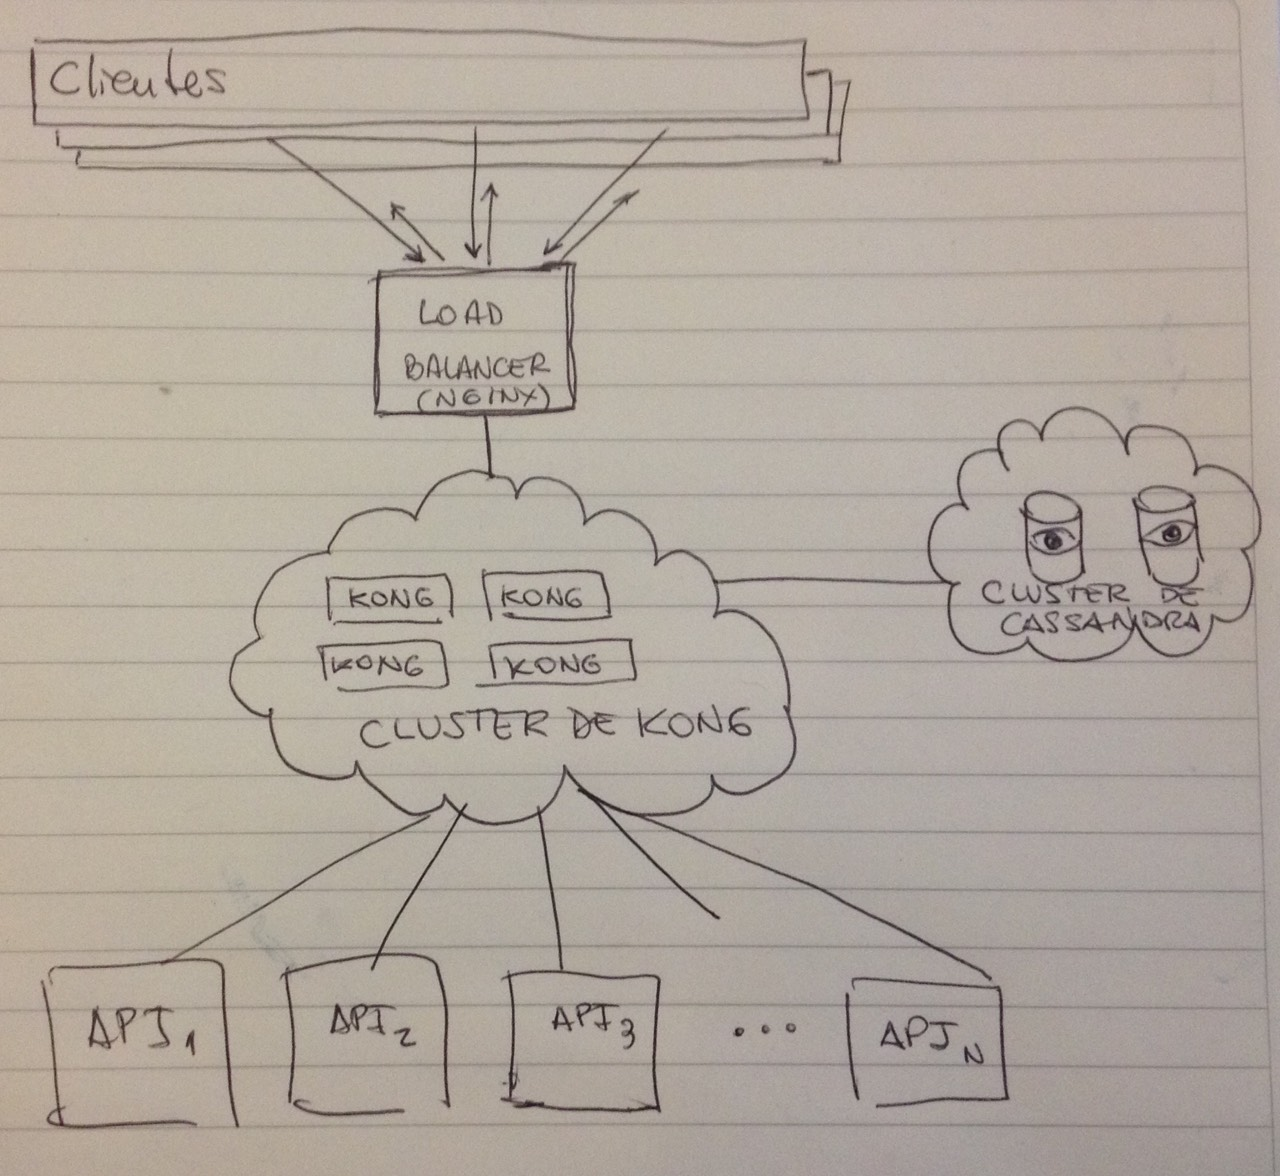
\includegraphics[width=\linewidth]{src/images/02-capitulo-2/tecnologias/kong/kong-arq.jpg}
  \caption{Esquema de integración de Kong en nuestra propuesta}
  \label{fig:integracion-kong-arquitectura}
\end{figure}

En nuestra arquitectura, tendríamos inicialmente un balanceador de carga delante de un cluster de instancias de Kong (junto con su correspondiente cluster de bases Cassandra con al menos dos instancias en réplica) como fachada para todas las peticiones a los servicios de la nube, y detrás de este tendríamos las distintas aplicaciones que proveen los \glspl{term:endpoint} específicos. En caso de necesitar escalar, bastará con agregar más instancias al cluster de Kong y, de ser necesario, también al cluster de bases de datos Cassandra.

En su función de proxy reverso, este producto nos será de gran utilidad al transicionar de la nube actual a la que estamos diseñando en este trabajo: podríamos enrutar todas las peticiones del \eng{hostname} \texttt{api2.dataintegration.unlp.edu.ar} a los servicios de la nube anterior y dirigir a las \glspl{acro:api} de la nueva arquitectura aquellas que lleguen a \texttt{cloud.unlp.edu.ar}. De esta forma, la migración de las aplicaciones cliente a la nueva arquitectura sería gradual.
